\documentclass[letterpaper,10pt]{article}

\usepackage{enumitem}
\usepackage{titling}
\usepackage{listings}
\usepackage{url}
\usepackage{hyperref}
\usepackage{setspace}
\usepackage{subfig}
\usepackage{sectsty}
\usepackage{pdfpages}
\usepackage{colortbl}
\usepackage{multirow}
\usepackage{multicol}
\usepackage{relsize}
\usepackage{amsmath}
\usepackage{wasysym}
\usepackage{fancyvrb}
\usepackage[yyyymmdd]{datetime}
\usepackage{amsmath,amssymb,amsthm,graphicx,xspace}
\usepackage[titlenotnumbered,noend,noline]{algorithm2e}
\usepackage[compact]{titlesec}
\usepackage{XCharter}
\usepackage[T1]{fontenc}
\usepackage[scaled]{beramono}
\usepackage[normalem]{ulem}
\usepackage{booktabs}
\usepackage{tikz}
\usetikzlibrary{arrows,automata,shapes,trees,matrix,chains,scopes,positioning,calc}
\tikzstyle{block} = [rectangle, draw, fill=blue!20,
text width=2.5em, text centered, rounded corners, minimum height=2em]
\tikzstyle{bw} = [rectangle, draw, fill=blue!20,
text width=4em, text centered, rounded corners, minimum height=2em]

\definecolor{namerow}{cmyk}{.40,.40,.40,.40}
\definecolor{namecol}{cmyk}{.40,.40,.40,.40}
\renewcommand{\dateseparator}{-}

\let\LaTeXtitle\title
\renewcommand{\title}[1]{\LaTeXtitle{\textsf{#1}}}

\lstset{basicstyle=\footnotesize\ttfamily,breaklines=true}

\newcommand{\handout}[5]{
	\noindent
	\begin{center}
		\framebox{
			\vbox{
				\hbox to 5.78in { {\bf SE 350: Operating Systems } \hfill #2 }
				\vspace{4mm}
				\hbox to 5.78in { {\Large \hfill #4  \hfill} }
				\vspace{2mm}
				\hbox to 5.78in { {\em #3 \hfill \today} }
			}
		}
	\end{center}
	\vspace*{4mm}
}

\newcommand{\lecture}[3]{\handout{#1}{#2}{#3}{Lecture#1}}
\newcommand{\tuple}[1]{\ensuremath{\left\langle #1 \right\rangle}\xspace}

\newcommand{\Rplus}{\protect\hspace{-.1em}\protect\raisebox{.35ex}{\smaller{\smaller\textbf{+}}}}
\newcommand{\Cpp}{\mbox{C\Rplus\Rplus}\xspace}


\addtolength{\oddsidemargin}{-1.000in}
\addtolength{\evensidemargin}{-0.500in}
\addtolength{\textwidth}{2.0in}
\addtolength{\topmargin}{-1.000in}
\addtolength{\textheight}{1.75in}
\addtolength{\parskip}{\baselineskip}
\setlength{\parindent}{0in}
\renewcommand{\baselinestretch}{1.5}
\newcommand{\term}{Winter 2023}
\newcommand{\termnumeric}{1231}

\singlespace


\begin{document}

\lecture{ 33 --- File System Implementation }{\term}{Jeff Zarnett}

\section*{File System Implementation}
Now it is time to go behind the scenes of how the file system lives up to the interface we have just finished discussing. The implementation is somewhat complicated, and to keep the size of the problem manageable we will worry about storing files on hard disks. Hard disks themselves make a good choice for this: they are sufficiently large and sufficiently cheap, to start with, to store the data that we want to store. We can read an arbitrary part of the disk. Finally, we can write to the same part of disk as many times as we want (disks don't, at least on the time frames that we are concerned about, wear out). Recall also that disks operate on blocks which, in their physical representation, comprise one or more sectors.

Let us take a look at the layers of the file system's design, from~\cite{osc}. As we descend down the list we will get closer to the hardware and less abstraction.

\paragraph{The File System.} The file system user interface is intended for the convenience of the user and for application programmers. This is the level we have just examined in the previous topic; the more interesting part is what happens when we need to fulfill the promises that the file system makes.

\paragraph{I/O Control.} At the I/O control level, we are dealing with device drivers and interrupt handlers to transfer data. The inputs are fairly high-level commands, along the lines of ``read block 1234''. Its outputs are hardware specific-instructions to the hardware controller. Usually this is by writing bit patterns in the I/O controller memory.

\paragraph{Basic File System.} Despite the awful name, this is the level at which we start to deal with physical blocks on the disk. A physical block is identified by its numerical physical address: drive 0, cylinder 12, track 7, sector 1. This layer is also responsible for buffers and caches that are used to hold various commonly-accessed regions (e.g., the temporary directory). Yes, caching and buffers can appear in the hard disk as well, with performance improvements traded off against the risk of data loss if power is suddenly cut.

\paragraph{File Organization Module.} This module is aware of files and their logical and physical blocks. This translates a logical block address to a physical block address and keeps track of free space (unallocated blocks).

\paragraph{The Logical File System.} This last level is for managing metadata: file system structure, directory structure, and maintaining the file structure. File data is maintained in a \textit{file control block} (FCB). The UNIX term for this is \textit{inode} and it is the place where file info is stored: ownership, permissions, locations of the file contents.

\subsection*{Disk Organization}

Although there are a million different file systems (UFS, HFS+, ZFS, NTFS, ext3, FAT32...) that are all significantly different, there are some general principles that we can examine. A file system will need to keep track of the total number of blocks, the number and locations of free blocks, the directory structure, and the files themselves.

On at least one disk somewhere in the system, there will need to be some information about how to boot up the operating system. Not every disk has the operating system on it, but if there is an OS the boot loader is usually put in the first block. When the power button is pressed on the case, the BIOS starts up and transfers control to whatever is found at that first block (which is hopefully your boot loader that launches the OS, or gives you the option of which OS to start).

Disks may be split, logically, into several different areas, or \textit{partitions}. Accordingly, there will be a partition table (sometimes called the superblock or master file table) that indicates what part of the disk belongs to which partition. In the Windows world we often see the whole disk is in one logical partition (the C: drive, for example, taking the whole primary disk). In Linux we often see the disk divided up to have partitions for different things: temporary/swap directory, home directories, boot partition, et cetera...

There are several structures that are likely to be in memory for performance reasons~\cite{osc}:

\begin{enumerate}
	\item \textbf{Mount Table}: Information about each mounted volume (disk/partition).
	\item \textbf{Cache}: Directory info for recently accessed directories.
	\item \textbf{Global Open File Table}: Copy of the FCB for each open file.
	\item \textbf{Process Open File Table}: References to the global open file table, sorted by process.
	\item \textbf{Buffers}: places where data read from or to be written to disk resides after or before the actual disk operation.
\end{enumerate}

Creating a new file is the job of the logical file system: allocation of a new FCB (or re-use of an existing free FCB). A typical FCB might look like this:

\begin{center}
	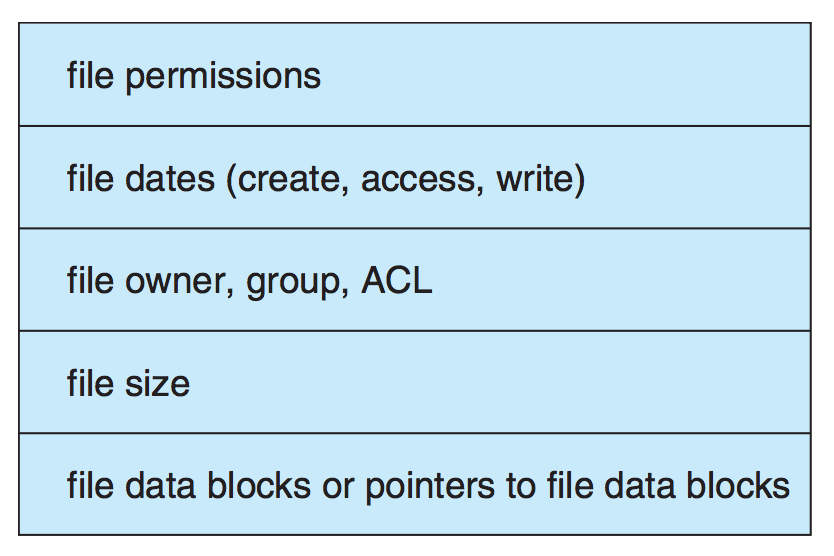
\includegraphics[width=0.4\textwidth]{images/fcb.png}\\
	File Control Block (FCB) example~\cite{osc}.
\end{center}

If a user (application) actually wants to make use of a file, the open system call is needed. Open operates on names, the user comprehensible version. The file system must then check the global open file table to see if the file is already open somewhere in the system. If so, if that file is opened for exclusive access, then the open routine returns with an error. If it is open but for non-exclusive access, then there is no need to search for the file or retrieve it by directory; we just make another reference in the process open file table. If the file is not already open, then it needs to be retrieved; once the file is found, the FCB is copied into the global open file table and the appropriate reference is added to the process table~\cite{osc}.

The process open file table can contain some additional information, like the next section to read or write, the access mode when the file is open, and so on. The open system call returns a pointer to the file table and this is the route through which the application performs all file operations. In UNIX this reference is called a \textit{file descriptor}; in Windows it is called a \textit{file handle}~\cite{osc}.

The opposite operation to opening a file is obviously to close it. When a process closes a file, the entry from the process open file table can be removed. If this is the last reference to the file a process has, then the file can also be removed from the global open file table. Metadata may be updated on close.

\paragraph{Searching with Spotlight.}

A small aside on the subject of metadata.

An example from Mac OS~X: the Spotlight system-wide desktop search. Spotlight was introduced quite some time ago but it was a revelation compared to the previous search options that were slow and did not necessarily include the file content, just the file names. Spotlight runs queries quickly over the metadata of the system. Spotlight examines each file on creation and modification and uses it to update the metadata related to that file. Those items are then added to the Spotlight index which can be queried very rapidly~\cite{spotlight}.

This is a specific case of preparing the data in advance to make searching or exporting operations fast. Another example is in exporting data to Excel. To export this data, there are two possible ways to do it. One is to examine and process the data for the Excel file at the time of the user request. The other is to maintain that data separately, and when the Excel report is asked for, take that data and put it in the Excel file.

Part of the difficulty with maintaining metadata is when to update it. The longer the time between metadata updates, the higher the chance that there will be a user request that gets back out-of-date data. The faster the metadata updates, the more time and processing power is spent creating and updating this metadata.

The diagram below shows how a file is opened and how a read takes place:

\begin{center}
	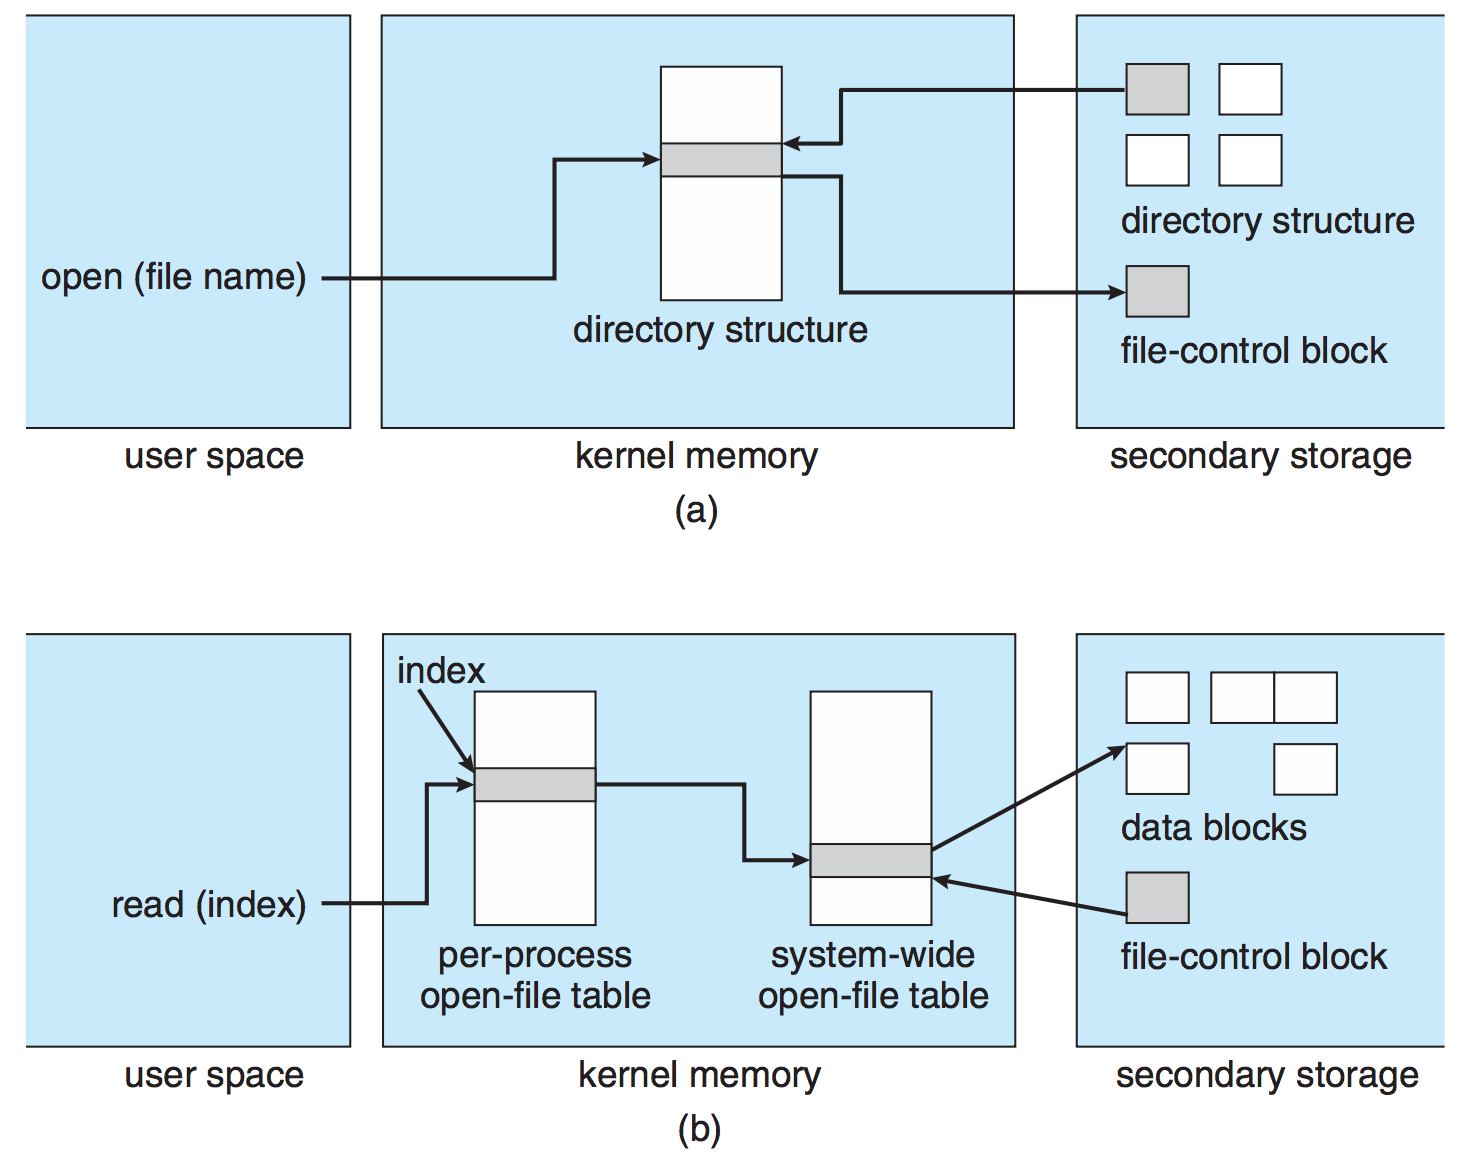
\includegraphics[width=0.75\textwidth]{images/file-system-structures.png}\\
	File System Structures for (a) file open and (b) file read~\cite{osc}.
\end{center}

\subsection*{Virtual File System}

We mentioned earlier that there are a lot of different file systems, like ext3, ZFS, etc. These may co-exist in the same system, though a partition will be formatted in only one of them. From the user's perspective, however, these operate identically. This is because of an additional layer of abstraction, called the virtual file system (VFS). 

There are two main purposes to the VFS. The first is to separate the file system operations (like reading, writing, opening, and closing files) from the actual implementation; thus operations can be done with whatever file system is actually implemented. The second is that it provides a mechanism for representing a file, uniquely, throughout a network. The file representation structure is called a \textit{vnode}, which is rather like an inode, but inodes are unique only within one file system. The VFS distinguishes between local and remote files~\cite{osc}.

\begin{center}
	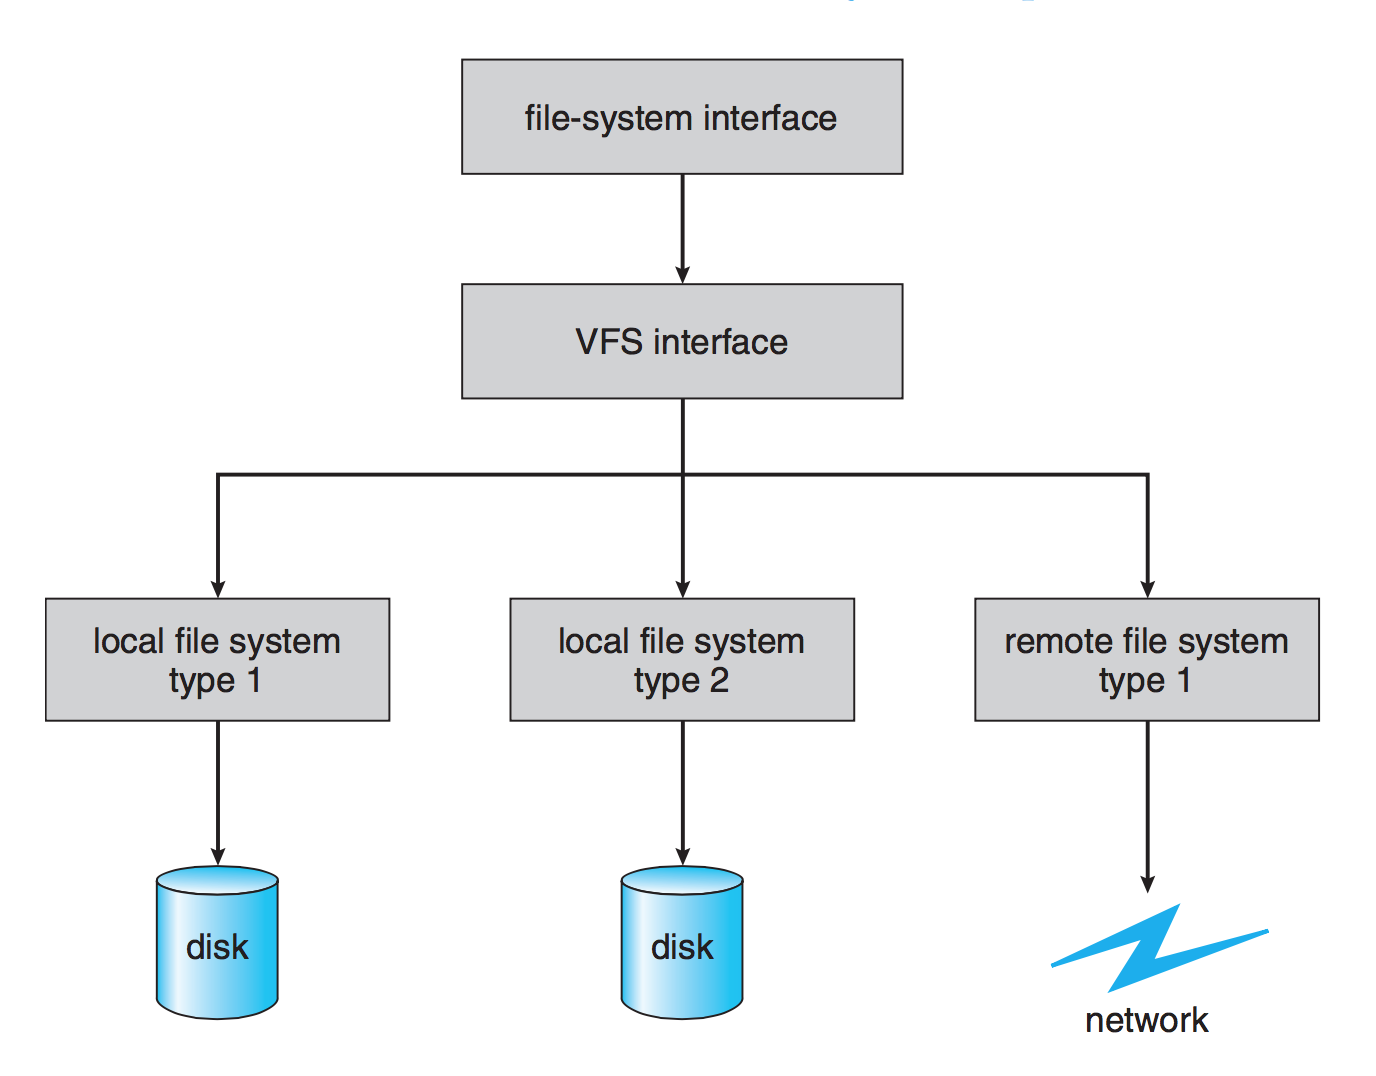
\includegraphics[width=0.5\textwidth]{images/vfs.png}\\
	Schematic view of the VFS Interface~\cite{osc}.
\end{center}

The VFS architecture in Linux has four main objects~\cite{osc}:
\begin{enumerate}
	\item inode (an individual file)
	\item file (an open file)
	\item superblock (the file system)
	\item dentry (a directory entry)
\end{enumerate}

For each of those, there are a set of operations defined. In the Linux kernel, these operations are defined in the \texttt{fs.h} headers and may include functions such as:

\begin{verbatim}
 ssize_t (*read) (struct file *, char __user *, size_t, loff_t *);
 ssize_t (*write) (struct file *, const char __user *, size_t, loff_t *);
 int (*open) (struct inode *, struct file *);
 int (*flush) (struct file *, fl_owner_t id);
 int (*release) (struct inode *, struct file *);
\end{verbatim}

The VFS therefore abstracts away a lot of the details of the underlying file system implementation.

\subsection*{Directory Implementation} 

See the table below for some information about what data may appear in a typical file directory.

\begin{center}
	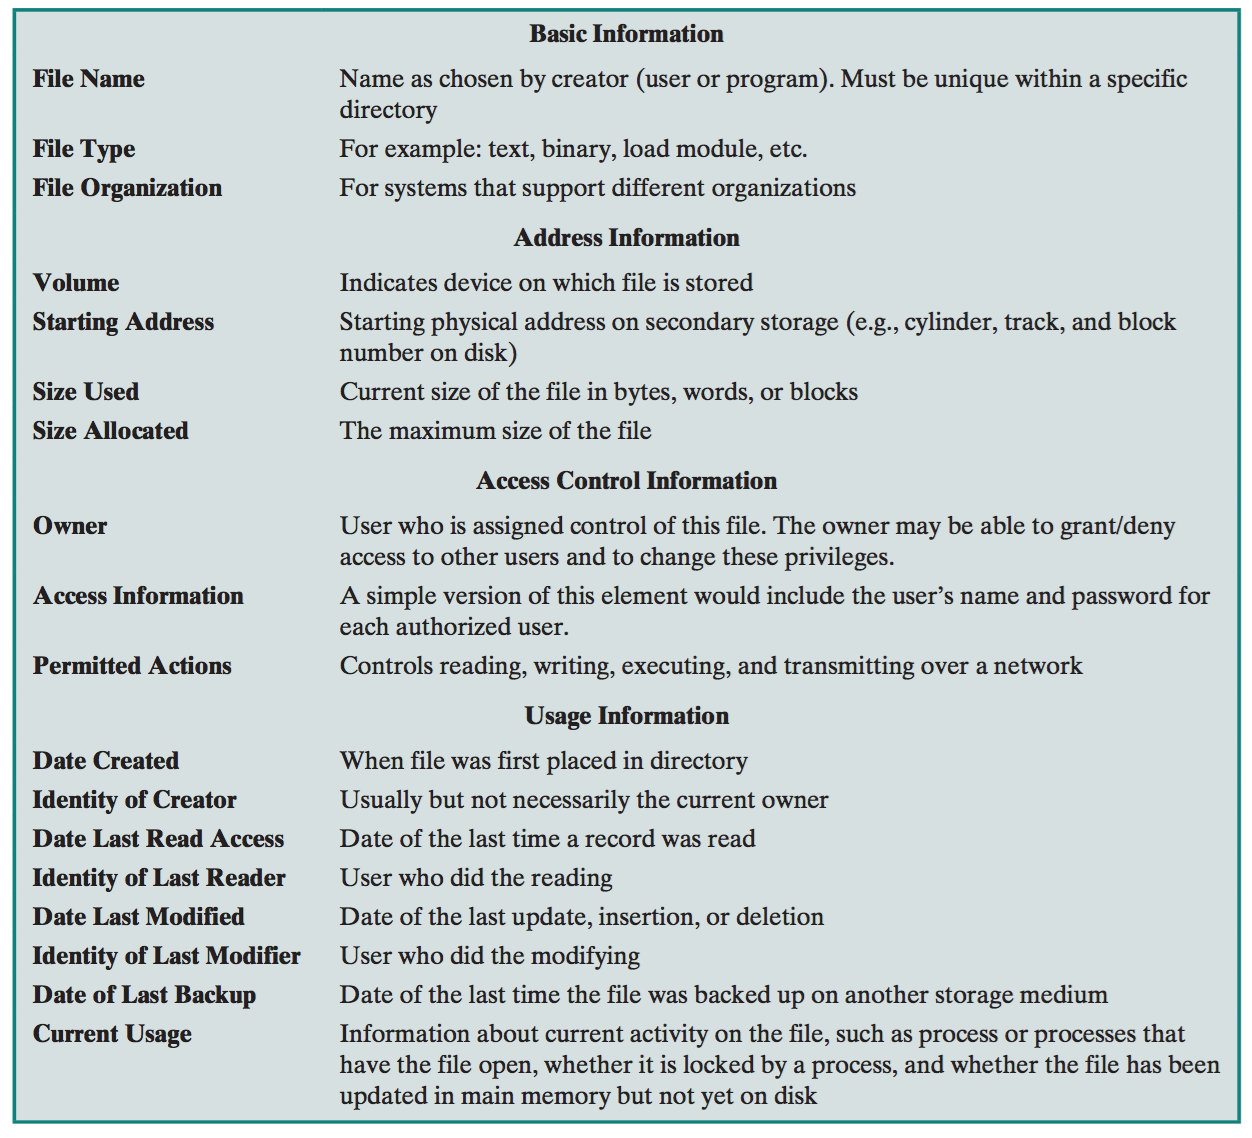
\includegraphics[width=0.75\textwidth]{images/directory.png}\\
	Information elements of a file directory~\cite{osi}.
\end{center}

A directory is, after all, not much beyond a set of files. And yet, there is a choice to be made in implementing them: a linear list versus a hash table. Both concepts should be familiar to you from data structures and algorithms.

The linear list option is certainly the simplest. Creating a new file requires searching the directory to see if there is a matching file name. If not, insert that new entry in the list. Deletion is also simple: search the list for the matching file and remove it; if it is the last reference to that file, we can free up the space. The real disadvantage to linear lists is that searching takes a long time. Searching through a directory can take quite a while, and the problem is compounded if the search is supposed to include the content of the file as well.

Alternatively, we could use a hash table. The hash is computed based on the file name, and of course there will need to be some strategy for dealing with hash collisions. Still, neither of these is satisfactory; what we really want is a more complex structure: a tree.

An AVL tree might be good as a way of storing ordered data, but it does not match well with the block system of a hard drive. Instead, we will examine a B-Tree, a variation on a binary search tree. 

Each node should occupy one block, so each node can contain a lot of information. File and directory information is linearly ordered, but a block does not need to be full. If a leaf node gets full, we can split it into two half-full blocks. Keeping the tree balanced means it takes about the same amount of time to find an item wherever it is.

A B-Tree structure, formally, has the following characteristics~\cite{osi}:

\begin{enumerate}
	\item The tree is made up of nodes (have children) and leaves (have no children).
	\item Each node contains at least one key identifying a file record, and more than one pointer to child nodes or child leaves.
	\item Each node has some maximum number of keys.
	\item The keys in a node are stored in non-decreasing order.
\end{enumerate}

And a B-tree of degree $d$ has the following properties~\cite{osi}:

\begin{enumerate}
	\item Every node has at most $2d-1$ keys and $2d$ children ($2d$ pointers).
	\item Every node other than the root has at least $d-1$ keys and $d$ pointers. Each internal node except the root is at least half full and has at least $d$ children.
	\item All leaves appear on the same level.
	\item A non-leaf node with $k$ pointers contains $k-1$ keys.
\end{enumerate}

To find something in a B-Tree, the general algorithm is fairly simple~\cite{osi}:

\begin{enumerate}
	\item Start at the root node. 
	\item If the key is in the current node, it is found, and the algorithm terminates.
	\item If the key is less than the smallest key in this node, follow the leftmost pointer; go to step 2.
	\item If the key is greater than the largest key in this node, follow the rightmost pointer; go to step 2.
	\item If the key is between the values of two adjacent keys, follow the pointer between them; go to step 2.
\end{enumerate}


Insertion into the B-Tree is more complicated, because of the rules that keep the tree balanced~\cite{osi}:

\begin{enumerate}
	\item Search the tree for the key. If it is not found, then we are at least looking at the block where it would be if it were there.
	\item If this node has fewer than $2d-1$ keys (that is, it is not full), insert the key into this node in the proper sequence. The algorithm terminates.
	\item If the node is full, split this node around the median key into two new nodes with $d-1$ keys each. Promote the median key to the higher level. If the new node is less than the median key, insert it in the left-hand new node; otherwise into the right.
	\item The promoted node is inserted into the parent node in order, splitting the parent if the parent is already full.
	\item If the process of promotion reaches the root node and the root is full, then splitting and promotion occurs and the height of the tree increases by 1.
\end{enumerate}

Some examples of how the insertion algorithm runs are shown below:

\begin{center}
	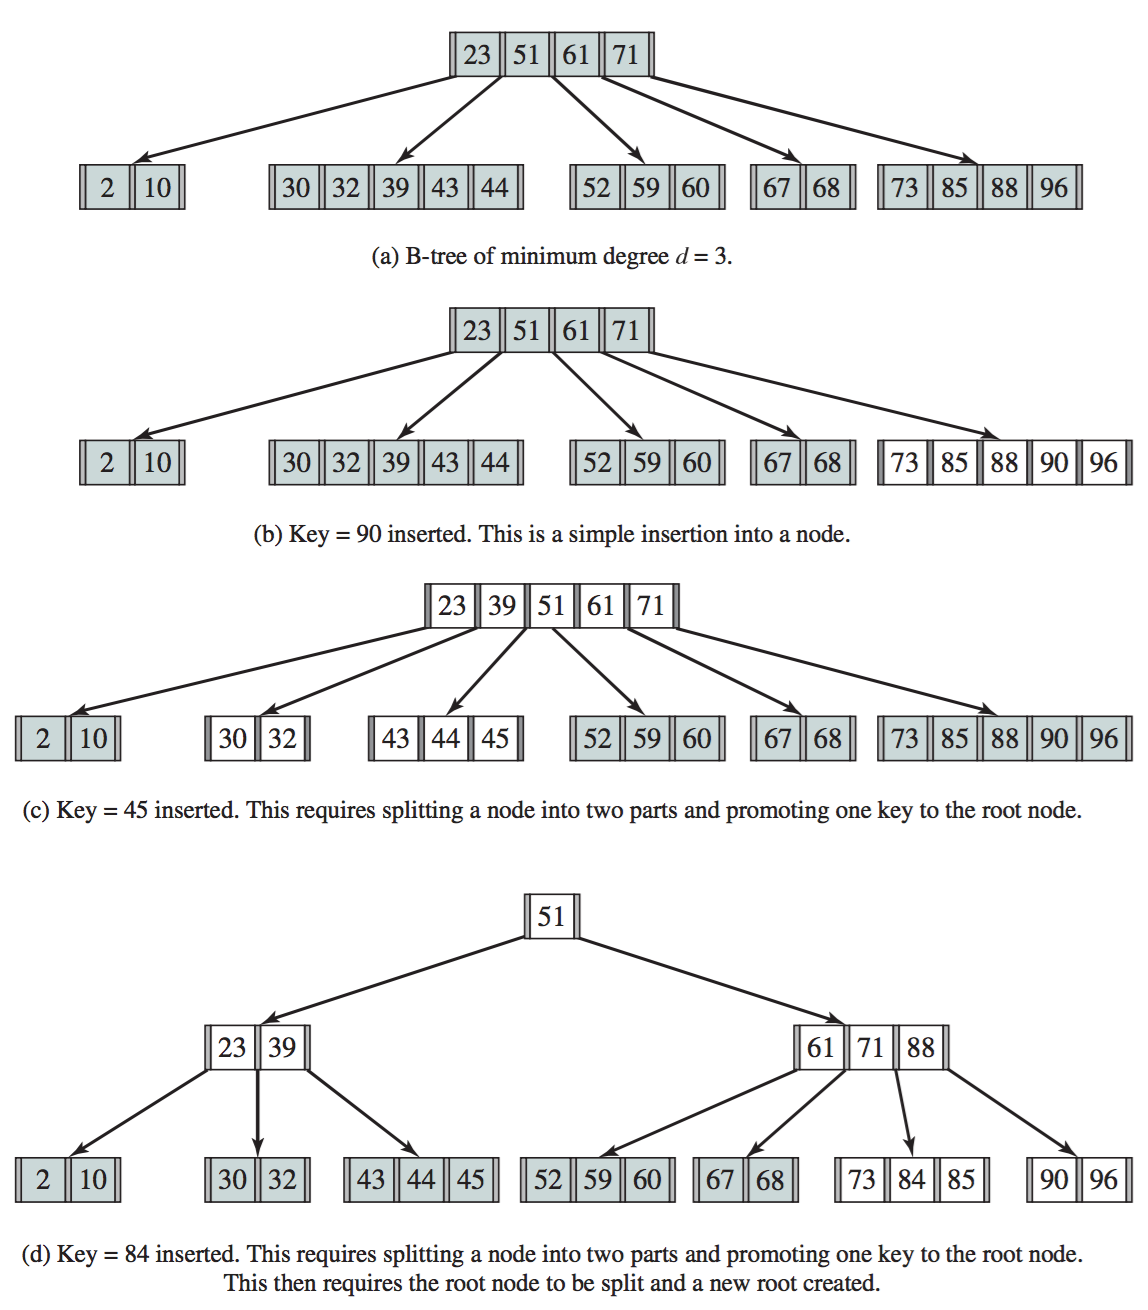
\includegraphics[width=0.9\textwidth]{images/b-tree-insert.png}\\
	Insertion of nodes 90, 45, and 84 into a B-Tree~\cite{osi}.
\end{center}

\bibliographystyle{alphaurl}
\bibliography{350}


\end{document}